\documentclass[twoside]{book}

% Packages required by doxygen
\usepackage{fixltx2e}
\usepackage{calc}
\usepackage{doxygen}
\usepackage[export]{adjustbox} % also loads graphicx
\usepackage{graphicx}
\usepackage[utf8]{inputenc}
\usepackage{makeidx}
\usepackage{multicol}
\usepackage{multirow}
\PassOptionsToPackage{warn}{textcomp}
\usepackage{textcomp}
\usepackage[nointegrals]{wasysym}
\usepackage[table]{xcolor}

% Font selection
\usepackage[T1]{fontenc}
\usepackage[scaled=.90]{helvet}
\usepackage{courier}
\usepackage{amssymb}
\usepackage{sectsty}
\renewcommand{\familydefault}{\sfdefault}
\allsectionsfont{%
  \fontseries{bc}\selectfont%
  \color{darkgray}%
}
\renewcommand{\DoxyLabelFont}{%
  \fontseries{bc}\selectfont%
  \color{darkgray}%
}
\newcommand{\+}{\discretionary{\mbox{\scriptsize$\hookleftarrow$}}{}{}}

% Page & text layout
\usepackage{geometry}
\geometry{%
  a4paper,%
  top=2.5cm,%
  bottom=2.5cm,%
  left=2.5cm,%
  right=2.5cm%
}
\tolerance=750
\hfuzz=15pt
\hbadness=750
\setlength{\emergencystretch}{15pt}
\setlength{\parindent}{0cm}
\setlength{\parskip}{3ex plus 2ex minus 2ex}
\makeatletter
\renewcommand{\paragraph}{%
  \@startsection{paragraph}{4}{0ex}{-1.0ex}{1.0ex}{%
    \normalfont\normalsize\bfseries\SS@parafont%
  }%
}
\renewcommand{\subparagraph}{%
  \@startsection{subparagraph}{5}{0ex}{-1.0ex}{1.0ex}{%
    \normalfont\normalsize\bfseries\SS@subparafont%
  }%
}
\makeatother

% Headers & footers
\usepackage{fancyhdr}
\pagestyle{fancyplain}
\fancyhead[LE]{\fancyplain{}{\bfseries\thepage}}
\fancyhead[CE]{\fancyplain{}{}}
\fancyhead[RE]{\fancyplain{}{\bfseries\leftmark}}
\fancyhead[LO]{\fancyplain{}{\bfseries\rightmark}}
\fancyhead[CO]{\fancyplain{}{}}
\fancyhead[RO]{\fancyplain{}{\bfseries\thepage}}
\fancyfoot[LE]{\fancyplain{}{}}
\fancyfoot[CE]{\fancyplain{}{}}
\fancyfoot[RE]{\fancyplain{}{\bfseries\scriptsize Generated by Doxygen }}
\fancyfoot[LO]{\fancyplain{}{\bfseries\scriptsize Generated by Doxygen }}
\fancyfoot[CO]{\fancyplain{}{}}
\fancyfoot[RO]{\fancyplain{}{}}
\renewcommand{\footrulewidth}{0.4pt}
\renewcommand{\chaptermark}[1]{%
  \markboth{#1}{}%
}
\renewcommand{\sectionmark}[1]{%
  \markright{\thesection\ #1}%
}

% Indices & bibliography
\usepackage{natbib}
\usepackage[titles]{tocloft}
\setcounter{tocdepth}{3}
\setcounter{secnumdepth}{5}
\makeindex

% Hyperlinks (required, but should be loaded last)
\usepackage{ifpdf}
\ifpdf
  \usepackage[pdftex,pagebackref=true]{hyperref}
\else
  \usepackage[ps2pdf,pagebackref=true]{hyperref}
\fi
\hypersetup{%
  colorlinks=true,%
  linkcolor=blue,%
  citecolor=blue,%
  unicode%
}

% Custom commands
\newcommand{\clearemptydoublepage}{%
  \newpage{\pagestyle{empty}\cleardoublepage}%
}

\usepackage{caption}
\captionsetup{labelsep=space,justification=centering,font={bf},singlelinecheck=off,skip=4pt,position=top}

%===== C O N T E N T S =====

\begin{document}

% Titlepage & ToC
\hypersetup{pageanchor=false,
             bookmarksnumbered=true,
             pdfencoding=unicode
            }
\pagenumbering{alph}
\begin{titlepage}
\vspace*{7cm}
\begin{center}%
{\Large Projeto1 \\[1ex]\large 1 }\\
\vspace*{1cm}
{\large Generated by Doxygen 1.8.13}\\
\end{center}
\end{titlepage}
\clearemptydoublepage
\pagenumbering{roman}
\tableofcontents
\clearemptydoublepage
\pagenumbering{arabic}
\hypersetup{pageanchor=true}

%--- Begin generated contents ---
\chapter{Projeto Cpp Fase 1}
\label{md__r_e_a_d_m_e}
\Hypertarget{md__r_e_a_d_m_e}
\subsection*{Collabs\+:}

Yawo Echitey Rafael Fernando Silva

\subsection*{Como executar\+:}

\subsubsection*{Usando o terminal(recomendado)}

Basta dar un clone no projeto e, acessando o diretorio do projeto usando o terminal, executar o comando \char`\"{}./main\char`\"{}. Caso queira recompilar de novo, executar os seguintes comandos\+: 
\begin{DoxyCode}
$ g++ -c ponto.cpp
$ g++ -c poligono.cpp
$ g++ -c retangulo.cpp
$ g++ -c main.cpp
$ g++ ponto.o poligono.o retangulo.o main.o -o main
$ ./main
\end{DoxyCode}


\subsubsection*{Usando o Qt\+:}

Basta criar um novo projeto, copiar os arquivos na pasta e executar pelo Qt. 
\chapter{Hierarchical Index}
\section{Class Hierarchy}
This inheritance list is sorted roughly, but not completely, alphabetically\+:\begin{DoxyCompactList}
\item \contentsline{section}{Point}{\pageref{class_point}}{}
\item \contentsline{section}{Poligono}{\pageref{class_poligono}}{}
\begin{DoxyCompactList}
\item \contentsline{section}{Retangulo}{\pageref{class_retangulo}}{}
\end{DoxyCompactList}
\end{DoxyCompactList}

\chapter{Class Index}
\section{Class List}
Here are the classes, structs, unions and interfaces with brief descriptions\+:\begin{DoxyCompactList}
\item\contentsline{section}{\hyperlink{class_point}{Point} }{\pageref{class_point}}{}
\item\contentsline{section}{\hyperlink{class_poligono}{Poligono} }{\pageref{class_poligono}}{}
\item\contentsline{section}{\hyperlink{class_retangulo}{Retangulo} }{\pageref{class_retangulo}}{}
\end{DoxyCompactList}

\chapter{File Index}
\section{File List}
Here is a list of all files with brief descriptions\+:\begin{DoxyCompactList}
\item\contentsline{section}{\hyperlink{main_8cpp}{main.\+cpp} }{\pageref{main_8cpp}}{}
\item\contentsline{section}{\hyperlink{poligono_8cpp}{poligono.\+cpp} }{\pageref{poligono_8cpp}}{}
\item\contentsline{section}{\hyperlink{poligono_8h}{poligono.\+h} }{\pageref{poligono_8h}}{}
\item\contentsline{section}{\hyperlink{ponto_8cpp}{ponto.\+cpp} }{\pageref{ponto_8cpp}}{}
\item\contentsline{section}{\hyperlink{ponto_8h}{ponto.\+h} }{\pageref{ponto_8h}}{}
\item\contentsline{section}{\hyperlink{retangulo_8cpp}{retangulo.\+cpp} }{\pageref{retangulo_8cpp}}{}
\item\contentsline{section}{\hyperlink{retangulo_8h}{retangulo.\+h} }{\pageref{retangulo_8h}}{}
\end{DoxyCompactList}

\chapter{Class Documentation}
\hypertarget{class_point}{}\section{Point Class Reference}
\label{class_point}\index{Point@{Point}}


{\ttfamily \#include $<$ponto.\+h$>$}

\subsection*{Public Member Functions}
\begin{DoxyCompactItemize}
\item 
\hyperlink{class_point_ad92f2337b839a94ce97dcdb439b4325a}{Point} ()
\item 
\hyperlink{class_point_a6524332fa4d321ff0a001366a732c7b6}{Point} (float \+\_\+x, float \+\_\+y)
\item 
void \hyperlink{class_point_a428a1676e2fdec6753c42011a1d59d18}{setX} (float \+\_\+x)
\item 
void \hyperlink{class_point_a9868c4601b0ea0c2d0de20fe41ee0e49}{setY} (float \+\_\+y)
\item 
void \hyperlink{class_point_ab5385c6d9bfa841e641e4709fc9f14cc}{set\+XY} (float \+\_\+x, float \+\_\+y)
\item 
float \hyperlink{class_point_acc27466778cc87a662bba40268c4c0c8}{getX} ()
\item 
float \hyperlink{class_point_a3cccbca94719ddde353cce86ce0e2f64}{getY} ()
\item 
\hyperlink{class_point}{Point} \hyperlink{class_point_a9dbea84b07b0a8ec3bbb9e58b3d15899}{add} (\hyperlink{class_point}{Point} p1)
\item 
\hyperlink{class_point}{Point} \hyperlink{class_point_a9cf2c53b0a4e6282a6712824bb4e9b00}{sub} (\hyperlink{class_point}{Point} p1)
\item 
float \hyperlink{class_point_abd2618d1f505d9392893273a66e7c9b2}{norma} ()
\item 
void \hyperlink{class_point_ad9676e36f3444534b609e3c68422239a}{translada} (float a, float b)
\item 
void \hyperlink{class_point_a1fb5c2501c27ab2cbc99d06c2a26a741}{imprime} ()
\end{DoxyCompactItemize}


\subsection{Constructor \& Destructor Documentation}
\mbox{\Hypertarget{class_point_ad92f2337b839a94ce97dcdb439b4325a}\label{class_point_ad92f2337b839a94ce97dcdb439b4325a}} 
\index{Point@{Point}!Point@{Point}}
\index{Point@{Point}!Point@{Point}}
\subsubsection{\texorpdfstring{Point()}{Point()}\hspace{0.1cm}{\footnotesize\ttfamily [1/2]}}
{\footnotesize\ttfamily Point\+::\+Point (\begin{DoxyParamCaption}{ }\end{DoxyParamCaption})}

\mbox{\Hypertarget{class_point_a6524332fa4d321ff0a001366a732c7b6}\label{class_point_a6524332fa4d321ff0a001366a732c7b6}} 
\index{Point@{Point}!Point@{Point}}
\index{Point@{Point}!Point@{Point}}
\subsubsection{\texorpdfstring{Point()}{Point()}\hspace{0.1cm}{\footnotesize\ttfamily [2/2]}}
{\footnotesize\ttfamily Point\+::\+Point (\begin{DoxyParamCaption}\item[{float}]{\+\_\+x,  }\item[{float}]{\+\_\+y }\end{DoxyParamCaption})}



\subsection{Member Function Documentation}
\mbox{\Hypertarget{class_point_a9dbea84b07b0a8ec3bbb9e58b3d15899}\label{class_point_a9dbea84b07b0a8ec3bbb9e58b3d15899}} 
\index{Point@{Point}!add@{add}}
\index{add@{add}!Point@{Point}}
\subsubsection{\texorpdfstring{add()}{add()}}
{\footnotesize\ttfamily \hyperlink{class_point}{Point} Point\+::add (\begin{DoxyParamCaption}\item[{\hyperlink{class_point}{Point}}]{p1 }\end{DoxyParamCaption})}

\mbox{\Hypertarget{class_point_acc27466778cc87a662bba40268c4c0c8}\label{class_point_acc27466778cc87a662bba40268c4c0c8}} 
\index{Point@{Point}!getX@{getX}}
\index{getX@{getX}!Point@{Point}}
\subsubsection{\texorpdfstring{get\+X()}{getX()}}
{\footnotesize\ttfamily float Point\+::getX (\begin{DoxyParamCaption}{ }\end{DoxyParamCaption})}

\mbox{\Hypertarget{class_point_a3cccbca94719ddde353cce86ce0e2f64}\label{class_point_a3cccbca94719ddde353cce86ce0e2f64}} 
\index{Point@{Point}!getY@{getY}}
\index{getY@{getY}!Point@{Point}}
\subsubsection{\texorpdfstring{get\+Y()}{getY()}}
{\footnotesize\ttfamily float Point\+::getY (\begin{DoxyParamCaption}{ }\end{DoxyParamCaption})}

\mbox{\Hypertarget{class_point_a1fb5c2501c27ab2cbc99d06c2a26a741}\label{class_point_a1fb5c2501c27ab2cbc99d06c2a26a741}} 
\index{Point@{Point}!imprime@{imprime}}
\index{imprime@{imprime}!Point@{Point}}
\subsubsection{\texorpdfstring{imprime()}{imprime()}}
{\footnotesize\ttfamily void Point\+::imprime (\begin{DoxyParamCaption}{ }\end{DoxyParamCaption})}

\mbox{\Hypertarget{class_point_abd2618d1f505d9392893273a66e7c9b2}\label{class_point_abd2618d1f505d9392893273a66e7c9b2}} 
\index{Point@{Point}!norma@{norma}}
\index{norma@{norma}!Point@{Point}}
\subsubsection{\texorpdfstring{norma()}{norma()}}
{\footnotesize\ttfamily float Point\+::norma (\begin{DoxyParamCaption}{ }\end{DoxyParamCaption})}

\mbox{\Hypertarget{class_point_a428a1676e2fdec6753c42011a1d59d18}\label{class_point_a428a1676e2fdec6753c42011a1d59d18}} 
\index{Point@{Point}!setX@{setX}}
\index{setX@{setX}!Point@{Point}}
\subsubsection{\texorpdfstring{set\+X()}{setX()}}
{\footnotesize\ttfamily void Point\+::setX (\begin{DoxyParamCaption}\item[{float}]{\+\_\+x }\end{DoxyParamCaption})}

\mbox{\Hypertarget{class_point_ab5385c6d9bfa841e641e4709fc9f14cc}\label{class_point_ab5385c6d9bfa841e641e4709fc9f14cc}} 
\index{Point@{Point}!set\+XY@{set\+XY}}
\index{set\+XY@{set\+XY}!Point@{Point}}
\subsubsection{\texorpdfstring{set\+X\+Y()}{setXY()}}
{\footnotesize\ttfamily void Point\+::set\+XY (\begin{DoxyParamCaption}\item[{float}]{\+\_\+x,  }\item[{float}]{\+\_\+y }\end{DoxyParamCaption})}

\mbox{\Hypertarget{class_point_a9868c4601b0ea0c2d0de20fe41ee0e49}\label{class_point_a9868c4601b0ea0c2d0de20fe41ee0e49}} 
\index{Point@{Point}!setY@{setY}}
\index{setY@{setY}!Point@{Point}}
\subsubsection{\texorpdfstring{set\+Y()}{setY()}}
{\footnotesize\ttfamily void Point\+::setY (\begin{DoxyParamCaption}\item[{float}]{\+\_\+y }\end{DoxyParamCaption})}

\mbox{\Hypertarget{class_point_a9cf2c53b0a4e6282a6712824bb4e9b00}\label{class_point_a9cf2c53b0a4e6282a6712824bb4e9b00}} 
\index{Point@{Point}!sub@{sub}}
\index{sub@{sub}!Point@{Point}}
\subsubsection{\texorpdfstring{sub()}{sub()}}
{\footnotesize\ttfamily \hyperlink{class_point}{Point} Point\+::sub (\begin{DoxyParamCaption}\item[{\hyperlink{class_point}{Point}}]{p1 }\end{DoxyParamCaption})}

\mbox{\Hypertarget{class_point_ad9676e36f3444534b609e3c68422239a}\label{class_point_ad9676e36f3444534b609e3c68422239a}} 
\index{Point@{Point}!translada@{translada}}
\index{translada@{translada}!Point@{Point}}
\subsubsection{\texorpdfstring{translada()}{translada()}}
{\footnotesize\ttfamily void Point\+::translada (\begin{DoxyParamCaption}\item[{float}]{a,  }\item[{float}]{b }\end{DoxyParamCaption})}



The documentation for this class was generated from the following files\+:\begin{DoxyCompactItemize}
\item 
\hyperlink{ponto_8h}{ponto.\+h}\item 
\hyperlink{ponto_8cpp}{ponto.\+cpp}\end{DoxyCompactItemize}

\hypertarget{class_poligono}{}\section{Poligono Class Reference}
\label{class_poligono}\index{Poligono@{Poligono}}


{\ttfamily \#include $<$poligono.\+h$>$}

Inheritance diagram for Poligono\+:\begin{figure}[H]
\begin{center}
\leavevmode
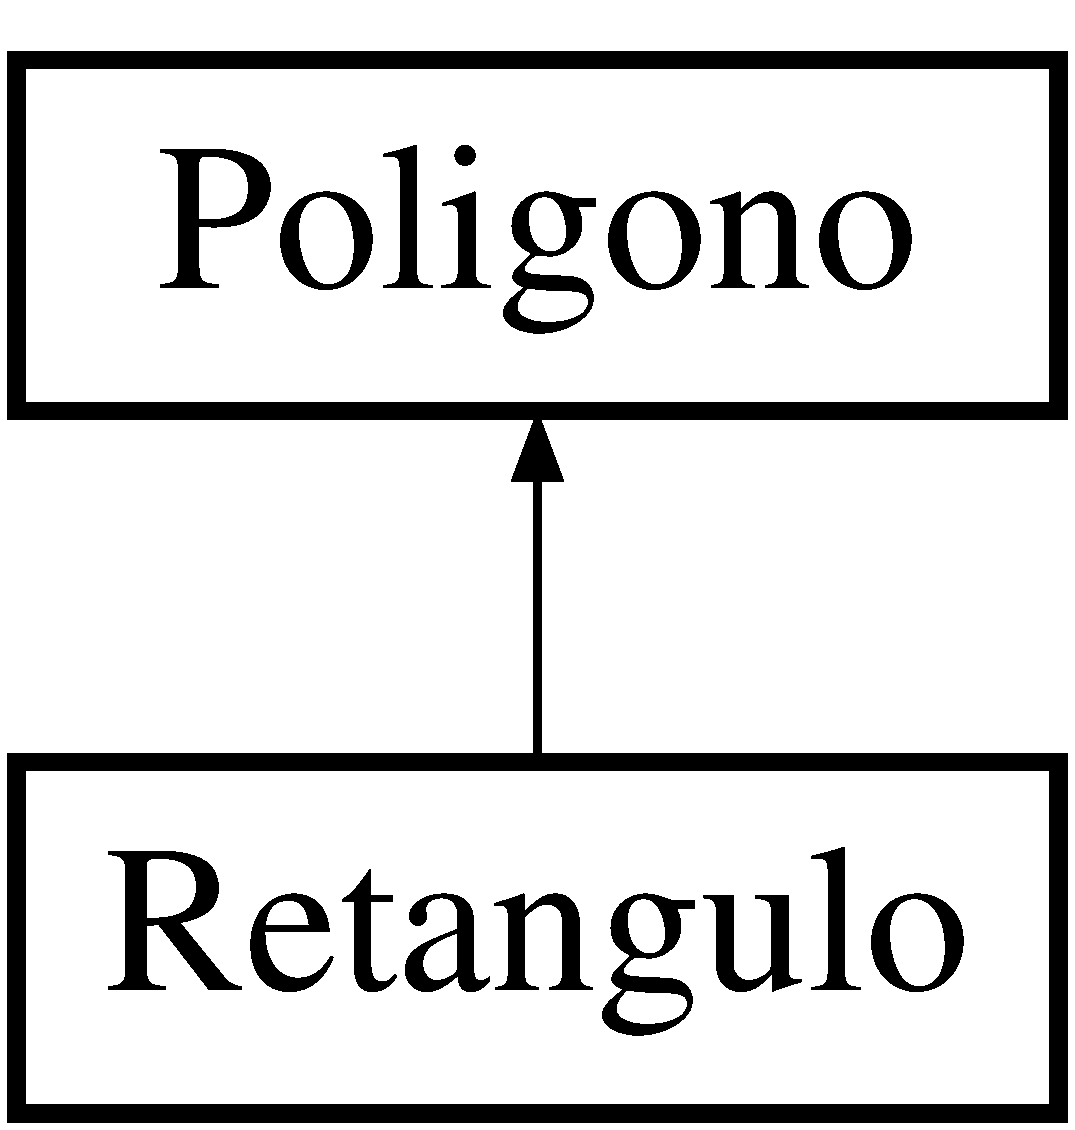
\includegraphics[height=2.000000cm]{class_poligono}
\end{center}
\end{figure}
\subsection*{Public Member Functions}
\begin{DoxyCompactItemize}
\item 
void \hyperlink{class_poligono_a49041ab4bc9ec5edb5a537c2ffd2ee11}{add\+Vertice} (float x, float y)
\item 
int \hyperlink{class_poligono_a84ebaf60416645892d91d1eb171e0442}{get\+Index} ()
\item 
\hyperlink{class_point}{Point} \hyperlink{class_poligono_a44c44b946558ffd10179d101bb9017ec}{get\+Origin} ()
\item 
int \hyperlink{class_poligono_ae4022d848bf0c3a4d4e3868ae4402250}{count} ()
\item 
float \hyperlink{class_poligono_a7f66c446f86c19118663ef1b2c8a4be6}{area} ()
\item 
void \hyperlink{class_poligono_adbf605dfd0419b7301c9be0ec1dbe41b}{translada} (float a, float b)
\item 
void \hyperlink{class_poligono_a793b09b4f7cfd02930318521d008362d}{rotacionar} (float angulo, \hyperlink{class_point}{Point} p)
\item 
void \hyperlink{class_poligono_a754dee9ed6a8fee4eb1a9d0aa0e1707a}{imprimir} ()
\end{DoxyCompactItemize}


\subsection{Member Function Documentation}
\mbox{\Hypertarget{class_poligono_a49041ab4bc9ec5edb5a537c2ffd2ee11}\label{class_poligono_a49041ab4bc9ec5edb5a537c2ffd2ee11}} 
\index{Poligono@{Poligono}!add\+Vertice@{add\+Vertice}}
\index{add\+Vertice@{add\+Vertice}!Poligono@{Poligono}}
\subsubsection{\texorpdfstring{add\+Vertice()}{addVertice()}}
{\footnotesize\ttfamily void Poligono\+::add\+Vertice (\begin{DoxyParamCaption}\item[{float}]{x,  }\item[{float}]{y }\end{DoxyParamCaption})}

\mbox{\Hypertarget{class_poligono_a7f66c446f86c19118663ef1b2c8a4be6}\label{class_poligono_a7f66c446f86c19118663ef1b2c8a4be6}} 
\index{Poligono@{Poligono}!area@{area}}
\index{area@{area}!Poligono@{Poligono}}
\subsubsection{\texorpdfstring{area()}{area()}}
{\footnotesize\ttfamily float Poligono\+::area (\begin{DoxyParamCaption}{ }\end{DoxyParamCaption})}

\mbox{\Hypertarget{class_poligono_ae4022d848bf0c3a4d4e3868ae4402250}\label{class_poligono_ae4022d848bf0c3a4d4e3868ae4402250}} 
\index{Poligono@{Poligono}!count@{count}}
\index{count@{count}!Poligono@{Poligono}}
\subsubsection{\texorpdfstring{count()}{count()}}
{\footnotesize\ttfamily int Poligono\+::count (\begin{DoxyParamCaption}{ }\end{DoxyParamCaption})}

\mbox{\Hypertarget{class_poligono_a84ebaf60416645892d91d1eb171e0442}\label{class_poligono_a84ebaf60416645892d91d1eb171e0442}} 
\index{Poligono@{Poligono}!get\+Index@{get\+Index}}
\index{get\+Index@{get\+Index}!Poligono@{Poligono}}
\subsubsection{\texorpdfstring{get\+Index()}{getIndex()}}
{\footnotesize\ttfamily int Poligono\+::get\+Index (\begin{DoxyParamCaption}{ }\end{DoxyParamCaption})}

\mbox{\Hypertarget{class_poligono_a44c44b946558ffd10179d101bb9017ec}\label{class_poligono_a44c44b946558ffd10179d101bb9017ec}} 
\index{Poligono@{Poligono}!get\+Origin@{get\+Origin}}
\index{get\+Origin@{get\+Origin}!Poligono@{Poligono}}
\subsubsection{\texorpdfstring{get\+Origin()}{getOrigin()}}
{\footnotesize\ttfamily \hyperlink{class_point}{Point} Poligono\+::get\+Origin (\begin{DoxyParamCaption}{ }\end{DoxyParamCaption})}

\mbox{\Hypertarget{class_poligono_a754dee9ed6a8fee4eb1a9d0aa0e1707a}\label{class_poligono_a754dee9ed6a8fee4eb1a9d0aa0e1707a}} 
\index{Poligono@{Poligono}!imprimir@{imprimir}}
\index{imprimir@{imprimir}!Poligono@{Poligono}}
\subsubsection{\texorpdfstring{imprimir()}{imprimir()}}
{\footnotesize\ttfamily void Poligono\+::imprimir (\begin{DoxyParamCaption}{ }\end{DoxyParamCaption})}

\mbox{\Hypertarget{class_poligono_a793b09b4f7cfd02930318521d008362d}\label{class_poligono_a793b09b4f7cfd02930318521d008362d}} 
\index{Poligono@{Poligono}!rotacionar@{rotacionar}}
\index{rotacionar@{rotacionar}!Poligono@{Poligono}}
\subsubsection{\texorpdfstring{rotacionar()}{rotacionar()}}
{\footnotesize\ttfamily void Poligono\+::rotacionar (\begin{DoxyParamCaption}\item[{float}]{angulo,  }\item[{\hyperlink{class_point}{Point}}]{p }\end{DoxyParamCaption})}

\mbox{\Hypertarget{class_poligono_adbf605dfd0419b7301c9be0ec1dbe41b}\label{class_poligono_adbf605dfd0419b7301c9be0ec1dbe41b}} 
\index{Poligono@{Poligono}!translada@{translada}}
\index{translada@{translada}!Poligono@{Poligono}}
\subsubsection{\texorpdfstring{translada()}{translada()}}
{\footnotesize\ttfamily void Poligono\+::translada (\begin{DoxyParamCaption}\item[{float}]{a,  }\item[{float}]{b }\end{DoxyParamCaption})}



The documentation for this class was generated from the following files\+:\begin{DoxyCompactItemize}
\item 
\hyperlink{poligono_8h}{poligono.\+h}\item 
\hyperlink{poligono_8cpp}{poligono.\+cpp}\end{DoxyCompactItemize}

\hypertarget{class_retangulo}{}\section{Retangulo Class Reference}
\label{class_retangulo}\index{Retangulo@{Retangulo}}


{\ttfamily \#include $<$retangulo.\+h$>$}

Inheritance diagram for Retangulo\+:\begin{figure}[H]
\begin{center}
\leavevmode
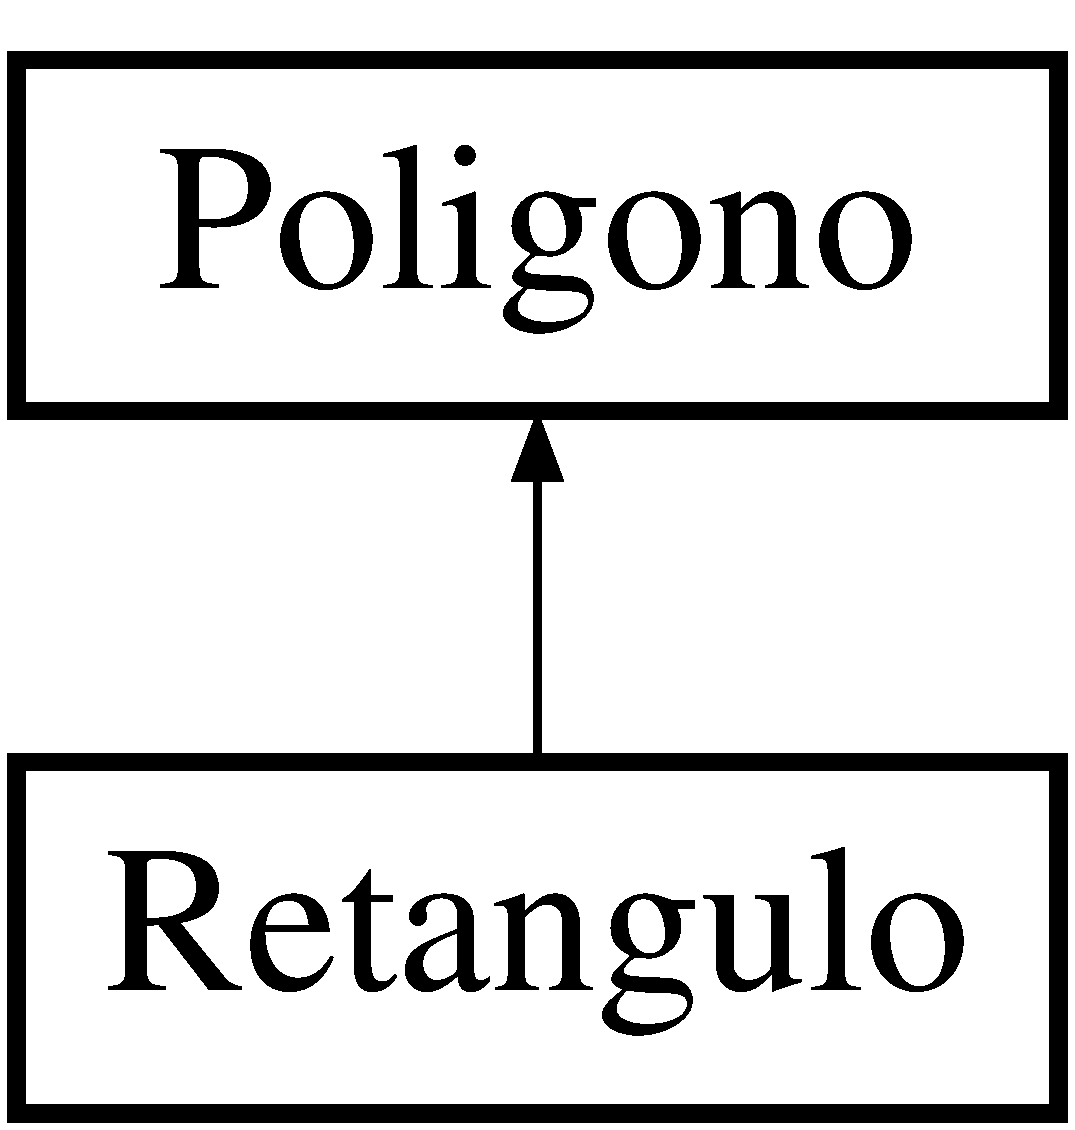
\includegraphics[height=2.000000cm]{class_retangulo}
\end{center}
\end{figure}
\subsection*{Public Member Functions}
\begin{DoxyCompactItemize}
\item 
\hyperlink{class_retangulo_acca1dd211eefc8dc04658c943c0d1122}{Retangulo} (float x, float y, float largura, float altura)
\end{DoxyCompactItemize}


\subsection{Constructor \& Destructor Documentation}
\mbox{\Hypertarget{class_retangulo_acca1dd211eefc8dc04658c943c0d1122}\label{class_retangulo_acca1dd211eefc8dc04658c943c0d1122}} 
\index{Retangulo@{Retangulo}!Retangulo@{Retangulo}}
\index{Retangulo@{Retangulo}!Retangulo@{Retangulo}}
\subsubsection{\texorpdfstring{Retangulo()}{Retangulo()}}
{\footnotesize\ttfamily Retangulo\+::\+Retangulo (\begin{DoxyParamCaption}\item[{float}]{x,  }\item[{float}]{y,  }\item[{float}]{largura,  }\item[{float}]{altura }\end{DoxyParamCaption})}



The documentation for this class was generated from the following files\+:\begin{DoxyCompactItemize}
\item 
\hyperlink{retangulo_8h}{retangulo.\+h}\item 
\hyperlink{retangulo_8cpp}{retangulo.\+cpp}\end{DoxyCompactItemize}

\chapter{File Documentation}
\hypertarget{main_8cpp}{}\section{main.\+cpp File Reference}
\label{main_8cpp}\index{main.\+cpp@{main.\+cpp}}
{\ttfamily \#include $<$iostream$>$}\newline
{\ttfamily \#include \char`\"{}ponto.\+h\char`\"{}}\newline
{\ttfamily \#include \char`\"{}retangulo.\+h\char`\"{}}\newline
{\ttfamily \#include \char`\"{}poligono.\+h\char`\"{}}\newline
\subsection*{Functions}
\begin{DoxyCompactItemize}
\item 
int \hyperlink{main_8cpp_ae66f6b31b5ad750f1fe042a706a4e3d4}{main} ()
\end{DoxyCompactItemize}


\subsection{Function Documentation}
\mbox{\Hypertarget{main_8cpp_ae66f6b31b5ad750f1fe042a706a4e3d4}\label{main_8cpp_ae66f6b31b5ad750f1fe042a706a4e3d4}} 
\index{main.\+cpp@{main.\+cpp}!main@{main}}
\index{main@{main}!main.\+cpp@{main.\+cpp}}
\subsubsection{\texorpdfstring{main()}{main()}}
{\footnotesize\ttfamily int main (\begin{DoxyParamCaption}{ }\end{DoxyParamCaption})}


\hypertarget{poligono_8cpp}{}\section{poligono.\+cpp File Reference}
\label{poligono_8cpp}\index{poligono.\+cpp@{poligono.\+cpp}}
{\ttfamily \#include $<$iostream$>$}\newline
{\ttfamily \#include $<$cmath$>$}\newline
{\ttfamily \#include \char`\"{}ponto.\+h\char`\"{}}\newline
{\ttfamily \#include \char`\"{}poligono.\+h\char`\"{}}\newline

\hypertarget{poligono_8h}{}\section{poligono.\+h File Reference}
\label{poligono_8h}\index{poligono.\+h@{poligono.\+h}}
{\ttfamily \#include \char`\"{}ponto.\+h\char`\"{}}\newline
\subsection*{Classes}
\begin{DoxyCompactItemize}
\item 
class \hyperlink{class_poligono}{Poligono}
\end{DoxyCompactItemize}
\subsection*{Macros}
\begin{DoxyCompactItemize}
\item 
\#define \hyperlink{poligono_8h_a0240ac851181b84ac374872dc5434ee4}{N}~100
\end{DoxyCompactItemize}


\subsection{Macro Definition Documentation}
\mbox{\Hypertarget{poligono_8h_a0240ac851181b84ac374872dc5434ee4}\label{poligono_8h_a0240ac851181b84ac374872dc5434ee4}} 
\index{poligono.\+h@{poligono.\+h}!N@{N}}
\index{N@{N}!poligono.\+h@{poligono.\+h}}
\subsubsection{\texorpdfstring{N}{N}}
{\footnotesize\ttfamily \#define N~100}


\hypertarget{ponto_8cpp}{}\section{ponto.\+cpp File Reference}
\label{ponto_8cpp}\index{ponto.\+cpp@{ponto.\+cpp}}
{\ttfamily \#include $<$iostream$>$}\newline
{\ttfamily \#include $<$cmath$>$}\newline
{\ttfamily \#include \char`\"{}ponto.\+h\char`\"{}}\newline

\hypertarget{ponto_8h}{}\section{ponto.\+h File Reference}
\label{ponto_8h}\index{ponto.\+h@{ponto.\+h}}
\subsection*{Classes}
\begin{DoxyCompactItemize}
\item 
class \hyperlink{class_point}{Point}
\end{DoxyCompactItemize}

\hypertarget{_r_e_a_d_m_e_8md}{}\section{R\+E\+A\+D\+M\+E.\+md File Reference}
\label{_r_e_a_d_m_e_8md}\index{R\+E\+A\+D\+M\+E.\+md@{R\+E\+A\+D\+M\+E.\+md}}

\hypertarget{retangulo_8cpp}{}\section{retangulo.\+cpp File Reference}
\label{retangulo_8cpp}\index{retangulo.\+cpp@{retangulo.\+cpp}}
{\ttfamily \#include $<$iostream$>$}\newline
{\ttfamily \#include $<$cmath$>$}\newline
{\ttfamily \#include \char`\"{}ponto.\+h\char`\"{}}\newline
{\ttfamily \#include \char`\"{}poligono.\+h\char`\"{}}\newline
{\ttfamily \#include \char`\"{}retangulo.\+h\char`\"{}}\newline

\hypertarget{retangulo_8h}{}\section{retangulo.\+h File Reference}
\label{retangulo_8h}\index{retangulo.\+h@{retangulo.\+h}}
{\ttfamily \#include \char`\"{}poligono.\+h\char`\"{}}\newline
\subsection*{Classes}
\begin{DoxyCompactItemize}
\item 
class \hyperlink{class_retangulo}{Retangulo}
\end{DoxyCompactItemize}

%--- End generated contents ---

% Index
\backmatter
\newpage
\phantomsection
\clearemptydoublepage
\addcontentsline{toc}{chapter}{Index}
\printindex

\end{document}
